
\part*{Kräfte}


\section*{Massepunkte}

Massepunkte sind charakterisiert durch die Position $\vec{r}(t)$,
durch die Masse M und durch die Ladung Q.


\section*{Beschleunigung}

Die Beschleunigung einer Masser ergibt sich aus der Summe der internen
und externen Kräfte:
\begin{verse}
$\vec{a}=\frac{1}{m}\cdot(\sum\vec{F}_{intern}+\sum\vec{F}_{extern})$
\end{verse}

\section*{Gravitationskraft}
\begin{verse}
$\vec{F}_{12}=-\gamma\frac{M_{1}M_{2}}{|\vec{r}_{12}|^{2}}\vec{n}_{12}=$Kraft
auf Masse M1

$\vec{r}_{12}=\vec{r}_{1}-\vec{r}_{2}$

$\vec{n}_{12}=\frac{\vec{r}_{12}}{|\vec{r}_{12}|}=$Einheitsvektor
von Masse M2 zu Masse M1

$\gamma=6.67\cdot10^{-11}\left[\frac{Nm^{2}}{kg^{2}}\right]=$Gravitationskonstante
\end{verse}
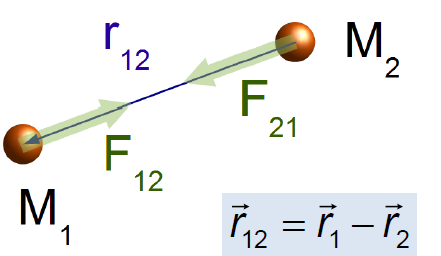
\includegraphics[scale=0.6]{Kräfte/Gravitation}


\subsection*{Superpositionsprinzip}

Die Gesamtkraft einer Anzahl von Massen auf eine bestimmte Masse ist
gleich der Summe der Kräfte der jeweiligen Einzelmassen.

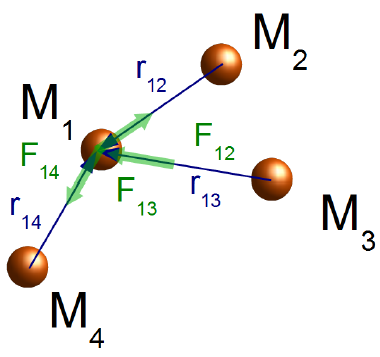
\includegraphics[scale=0.6]{Kräfte/Superpositionsprinzip}


\section*{Planetenbahnen}
\begin{verse}
$\vec{F}=-\gamma\frac{mM_{s}}{|\vec{r}|^{2}}\vec{n}\Rightarrow ma=\gamma\frac{mM_{s}}{r^{2}}$

$\vec{a}(t)=\left(\begin{array}{c}
-r\omega^{2}cos(\omega t)\\
-r\omega^{2}sin(\omega t)
\end{array}\right)\Rightarrow|\vec{a}(t)|=r\omega^{2}$

$\Rightarrow mr\omega^{2}=\gamma\frac{mM_{s}}{r^{2}}\Rightarrow r^{3}\omega^{2}=\gamma M_{s}$

m = Planetenmasse

$M_{s}$= Sonnenmasse

r = Radius der Kreisbahn
\end{verse}

\subsection*{Keppler's third law}
\begin{verse}
$\frac{r^{3}}{T^{2}}=\frac{\gamma M_{s}}{4\pi^{2}}=const.$

T = Periode = $\frac{2\pi}{\omega}$
\end{verse}

\section*{Elektrische Ladung}

Ein Elektron trägt eine Ladung von -e, wobei e die Elementarladung
$e=1.602189\cdot10^{-19}C$ beträgt.


\subsection*{Kräfte zwischen ruhenden Ladungen}

Gleiche Ladungen stossen sich ab, ungleiche ziehen sich an.
\begin{verse}
$\vec{F}=\frac{1}{4\pi\varepsilon_{0}}\cdot\frac{Q_{1}Q_{2}}{|\vec{r}_{12}|^{2}}\vec{n}_{12}$

$\varepsilon_{0}=8.859\cdot10^{-12}\left[\frac{C^{2}}{Jm}\right]=$Influenzkonstante
\end{verse}

\section*{Reibungskräfte}


\subsection*{Bodenkraft}

Die Gravitationskraft wird durch eine Kraft des Bodens, die ``Bodenkraft''
ausgeglichen.


\subsection*{Gleitreibung}
\begin{verse}
$\vec{F}_{G}=-\vec{F}_{B}$

$\vec{F}_{R}=-\mu\cdot m\cdot g\cdot\vec{n}_{v}$

$\vec{n}_{v}=\frac{\vec{v}}{|\vec{v}|}$

$\mu=$Gleitreibungskoeff.

$m=$Masse

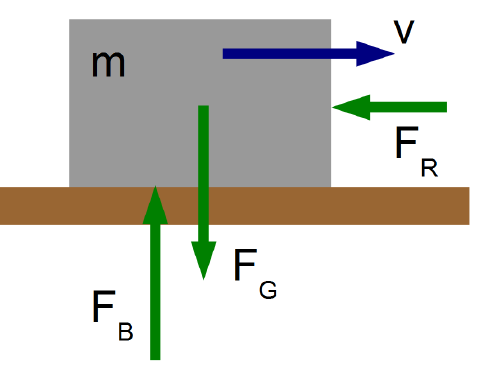
\includegraphics[scale=0.4]{Kräfte/Gleitreibung}
\end{verse}

\subsection*{Haftreibung}
\begin{verse}
$\vec{F}_{C}=\mu_{H}\cdot m\cdot g\cdot\vec{n}_{_{Fpull}}$

$\vec{F}_{R}=-\vec{F}_{pull}$(solange $\vec{F}_{pull}\leq\vec{F}_{C}$
und $\vec{v}=0$)

$\vec{n}_{Fpull}=\frac{\vec{F}_{pull}}{|\vec{F}_{pull}|}$

$\mu_{H}=$Haftreibungskoeffizient

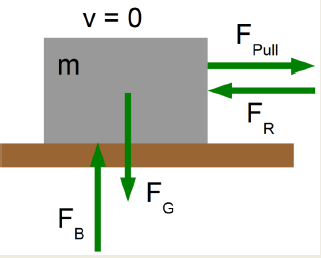
\includegraphics[scale=0.6]{Kräfte/Haftreibung}\end{verse}

